\begin{frame}
	\frametitle{Wie kommunizieren wir im Internet?}

	\begin{center}
		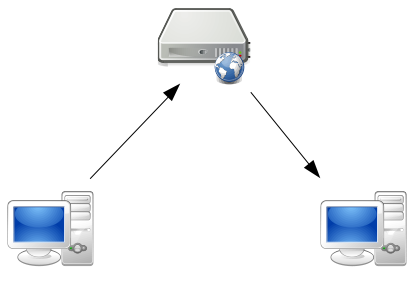
\includegraphics[height=5cm]{img/c-s.png}
	\end{center}
\end{frame}
\note{Stark vereinfacht kommunizieren zwei Internetnutzer, die sich eine Nachricht - beispielsweise über einen Messenger oder ein soziales Netzwerk - zusenden, indem der Sender die Nachrichten durchs Internet an einen Server schickt und dieser sie an den Empfänger weiterleitet. Ein Server ist ein Computer, der 24/7 angeschaltet ist und immer unter der selben Adresse im Internet zu finden ist.}

\begin{frame}
	\frametitle{Föderation}
	\begin{center}
		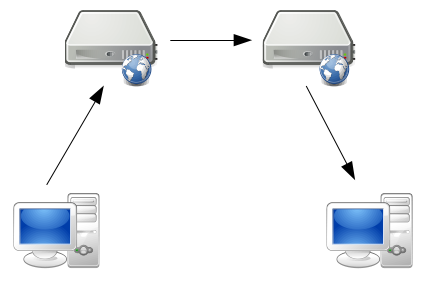
\includegraphics[height=5cm]{img/fed.png}
	\end{center}
\end{frame}

\note{Gelegentlich findet man im Internet auch das Föderationsmodell. Hier betreibt nicht eine Organisation den Dienst den alle nutzen (wie z.B. bei Facebook der Fall), sondern jeder Nutzer kann sich seinen Anbieter selbst aussuchen. Dies ist z.B. bei E-Mail, Jabber oder Nextcloud (eine Art persönlicher Dropbox/Google Contacts+Calendar/Apple iCloud-Ersatz) der Fall. Hier wird eine Nachricht/ein Datum/eine Datei erst an den eigenen Anbieter geschickt und der leitet sie dann an den Anbieter des Empfängers weiter.}
